% Options for packages loaded elsewhere
\PassOptionsToPackage{unicode}{hyperref}
\PassOptionsToPackage{hyphens}{url}
%
\documentclass[
]{article}
\usepackage{amsmath,amssymb}
\usepackage{iftex}
\ifPDFTeX
  \usepackage[T1]{fontenc}
  \usepackage[utf8]{inputenc}
  \usepackage{textcomp} % provide euro and other symbols
\else % if luatex or xetex
  \usepackage{unicode-math} % this also loads fontspec
  \defaultfontfeatures{Scale=MatchLowercase}
  \defaultfontfeatures[\rmfamily]{Ligatures=TeX,Scale=1}
\fi
\usepackage{lmodern}
\ifPDFTeX\else
  % xetex/luatex font selection
\fi
% Use upquote if available, for straight quotes in verbatim environments
\IfFileExists{upquote.sty}{\usepackage{upquote}}{}
\IfFileExists{microtype.sty}{% use microtype if available
  \usepackage[]{microtype}
  \UseMicrotypeSet[protrusion]{basicmath} % disable protrusion for tt fonts
}{}
\makeatletter
\@ifundefined{KOMAClassName}{% if non-KOMA class
  \IfFileExists{parskip.sty}{%
    \usepackage{parskip}
  }{% else
    \setlength{\parindent}{0pt}
    \setlength{\parskip}{6pt plus 2pt minus 1pt}}
}{% if KOMA class
  \KOMAoptions{parskip=half}}
\makeatother
\usepackage{xcolor}
\usepackage[margin=1in]{geometry}
\usepackage{graphicx}
\makeatletter
\def\maxwidth{\ifdim\Gin@nat@width>\linewidth\linewidth\else\Gin@nat@width\fi}
\def\maxheight{\ifdim\Gin@nat@height>\textheight\textheight\else\Gin@nat@height\fi}
\makeatother
% Scale images if necessary, so that they will not overflow the page
% margins by default, and it is still possible to overwrite the defaults
% using explicit options in \includegraphics[width, height, ...]{}
\setkeys{Gin}{width=\maxwidth,height=\maxheight,keepaspectratio}
% Set default figure placement to htbp
\makeatletter
\def\fps@figure{htbp}
\makeatother
\setlength{\emergencystretch}{3em} % prevent overfull lines
\providecommand{\tightlist}{%
  \setlength{\itemsep}{0pt}\setlength{\parskip}{0pt}}
\setcounter{secnumdepth}{-\maxdimen} % remove section numbering
\usepackage{titling}
\pretitle{\begin{center}\Huge\bfseries}
\posttitle{\par\end{center}}
\predate{\begin{center}\large}
\postdate{\par\end{center}}
\preauthor{\begin{center}\large}
\postauthor{\par\end{center}}
\usepackage{amsmath}
\usepackage{amsthm}
\usepackage{rotating}
\ifLuaTeX
  \usepackage{selnolig}  % disable illegal ligatures
\fi
\usepackage{bookmark}
\IfFileExists{xurl.sty}{\usepackage{xurl}}{} % add URL line breaks if available
\urlstyle{same}
\hypersetup{
  pdftitle={Transit Usage in Seattle: A Spatial Investigation},
  pdfauthor={Peter Silverstein},
  hidelinks,
  pdfcreator={LaTeX via pandoc}}

\title{Transit Usage in Seattle: A Spatial Investigation}
\author{Peter Silverstein}
\date{2024-12-10}

\begin{document}
\maketitle

\begin{center}
    {\large Final Project}\\[0.5cm]
    {\large GIS and Spatial Analysis}\\[0.5cm]
    {\large QMSS5070}\\[0.5cm]
\end{center}

\newpage

\section{Introduction}\label{introduction}

\subsection{Research Question:}\label{research-question}

\begin{enumerate}
\def\labelenumi{\arabic{enumi}.}
\tightlist
\item
  How does transit usage percentage (percent of trips using mass transit
  / total trips per census tract) vary spatially in and around Seattle
  and Tacoma, Washington?
\item
  How does this variation relate to population density, median income,
  and median age at the census tract level?
\end{enumerate}

\subsection{Purpose of Study:}\label{purpose-of-study}

There are essentially two purposes to this study. The first is to better
understand where there are concentrations of high and low transit usage
around the region. If there is clustering and we see hotspots and
coldspots, further policy-focused questions can be asked. For example:
given clustering, what characteristics of a census tract makes in more
or less likely to be in one of these hot or cold zones? How might we
allocate resources across hot zones, cold zones, and those in-between to
increase the adoption of transit by commuters? Is the dispersion of
transit availability closely related to the demand and does the
dispersion favor certain demographic groups over others?

The second research question is a very basic attempt at answering one of
these follow-up questions. By understanding how the three variables
(population density, median income, and median age) are related to the
outcome of interest (percentage of commuter trips taken using public
transit), we can begin to fill in the knowledge gaps demonstrated by the
questions above.

\subsection{Hypotheses}\label{hypotheses}

\begin{enumerate}
\def\labelenumi{\arabic{enumi}.}
\tightlist
\item
  I believe we will see transit hotspots close to urban centers (e.g.,
  Seattle and Tacoma, the two biggest cities in the region of interest).
  Further, I believe the opposite will be true for coldspots--they
  should exist further outside urban centers. These ideas are based on
  the fact that transit lines themselves tend to be clustered in
  high-density, urban areas, meaning opportunities for mass transit
  travel are more convenient and plentiful in more central urban areas.
\item
  I expect that transit use percentage is positively associated with
  population density and median income and negatively associated with
  age. I make this hypothesis about population density based on the
  reasoning above. I expect younger people to (a) be more likely to live
  in highly urban areas and (b) be less likely to own a personal vehicle
  (such as a car). Of the three variables, I am the least confident
  about median income, because I think the relationship could be pulled
  in both positive and negative directions. On one hand, urban areas
  tend to be more expensive and thus have a higher requirement for
  income to live there. On the other hand, lower income should be
  associated with lower rates of car ownership and thus lower income
  would be associated with higher transit ridership.
\end{enumerate}

\section{Data and Methodology:}\label{data-and-methodology}

\subsection{Data Sources:}\label{data-sources}

\begin{enumerate}
\def\labelenumi{\arabic{enumi}.}
\tightlist
\item
  The \textbf{Puget Sound Regional Association (PSRC) Household Travel
  Survey (HTS) 2017-23} is a biennial survey of commuters done in the
  King, Kitsap, Pierce, and Snohomish counties of Washington state (the
  counties surrounding Seattle and Tacoma). The present analysis uses
  the Trips dataset from the HTS. Each observation in the dataset
  represents a single trip taken by a respondent and includes a variety
  of variables. Most important for my analysis are origin/destination
  tract and mode of travel, although the dataset also includes date,
  time, distance, speed, etc.
\item
  All \textbf{census tract-level ACS 2022 5-year estimates for
  demographic data and the associated geometries} were accessed via the
  R \texttt{tidycensus} package, which leverages an API connection to
  the US Census Bureau to provide US Census data for a specified
  geographic area.
\item
  Finally, \textbf{Stanford's Cities and Towns of the United States,
  2014} dataset provided point data to allow me to add city labels to my
  maps for reference.
\end{enumerate}

\subsection{Data Preparation/Spatial Data
Management:}\label{data-preparationspatial-data-management}

\subsubsection{Data Cleaning}\label{data-cleaning}

The output from \texttt{tidycensus} is already quite clean, so the
majority of data cleaning steps were conducted on the PSRC HTS dataset.
After loading the dataset, I selected my columns of interest and
converted their types where appropriate and useful (e.g., string to
factor). The next step was to collapse the mode of travel column from
around 50 unique responses (an artifact of (a) a very detailed survey
and (b) some option changes over the years of the survey) to just 4
useful categories, outlined below:

\begin{enumerate}
\def\labelenumi{\arabic{enumi}.}
\tightlist
\item
  \emph{Mass Transit:} included in this category trips that used a metro
  bus, private bus or shuttle, urban rail/light rail, school bus, ferry,
  paratransit, and commuter rail. Essentially I included any
  multi-occupancy transit vehicle.
\item
  \emph{Personal Vehicle:} trips including all single-occupancy motor
  vehicles. This includes personal cars, ride-shares, taxis,
  motorcycles, and car-share services.
\item
  \emph{Active Transit:} included walking, running, biking, and
  skateboarding.
\item
  \emph{Other:} included helicopter/plane, ``other'' responses.
\end{enumerate}

I then implemented a number of filters to filter data that didn't pass
muster for realism/were outside the scope of this question. This
included the following operations:

\begin{enumerate}
\def\labelenumi{\arabic{enumi}.}
\tightlist
\item
  Filtered non-complete survey responses
\item
  Filtered distance to the range of 0 to 150 miles
\item
  Filtered trip duration to only include those greater than 0 minutes
\item
  Filtered speed to exclude speeds greater than 150 mph
\item
  Filtered to remove observations with missing value for travel mode
\end{enumerate}

\subsubsection{Spatial Joins}\label{spatial-joins}

The next step was to count the number of trips and join these values to
the geometries/ACS data from tidyverse. I used the \texttt{summarize()}
function to count the number of total trips and number of trips per
category for each census tracts. I then joined these counts to my
geometry table via the \texttt{left\_join()} function and matched on
GEOID. Further, I removed any tracts from the analysis with 0 total
trips. I acknowledge that this is a bit of a simplistic solution to
missingness and will discuss it further in my analysis and conclusions.
Finally, I calculated the percentage of trips in each tract that were
made by mass transit mode (count of mass transit / count of total
trips).

\subsection{GIS Methodology Overview}\label{gis-methodology-overview}

\subsubsection{Manipulation/Analytical Methods
Used}\label{manipulationanalytical-methods-used}

As mentioned above, I counted the number of trips inside each census
tract, then converted the total trip and mass transit trip counts to
percentage. Finally, I used a simple join function to associate the
counts with their respective geometries.

For the analysis in this project, I will perform a global cluster
analysis (using Moran's I) and visualize any hot and cold zones using
Getis-Ord Gi*. These approaches should help me understand whether
transit use is clustered and visualize where it is clustered. I will
then run a Spatial Error Model (SEM) and a Spatial Lag Model (SLM)
regressing mass transit percentage on population density, median income,
and median age. I believe that the SEM is the better conceptual choice -
I believe that it is likely that unmeasured factors (e.g., land use,
transit quality/reliability, parking availability) are spatially
correlated, while the idea that ridership in one tract influences
another is a bit harder to intuit. That said, I will run both models in
order to compare the results.

\subsubsection{Software Used}\label{software-used}

All data loading, cleaning, and manipulation, mapping (both choropleth
and Getis-Ord Gi*), table-creation, regression modeling, and write-up
were performed with R and R-Studio.

\newpage

\section{Results and Analysis}\label{results-and-analysis}

\subsection{Exploratory Data Analysis via Choropleth Mapping and
Descriptive
Tables}\label{exploratory-data-analysis-via-choropleth-mapping-and-descriptive-tables}

I will begin the analysis portion of this project with some simple
choropleth maps. The purpose of this mapping is to simply visualize the
spatial patterning of the dependent and independent variables. While the
actual significance testing and cluster analysis will give us a
scientific understanding of the problem, many of the patterns we're
looking for will be apparent with a simple eye test.

\begin{figure}
\centering
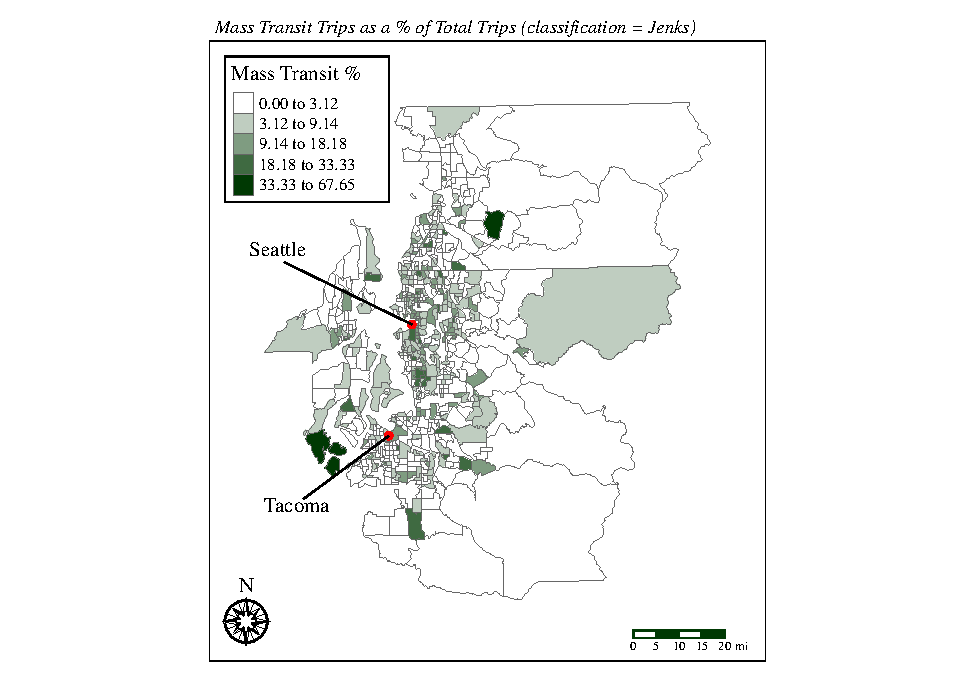
\includegraphics{transit-hotspots-PSRC_files/figure-latex/unnamed-chunk-3-1.pdf}
\caption{Sources: US Census ACS 2022 5-year estimates, Puget Sound
Regional Countil, Cities and Towns of the US 2014, via Stanford
University; Classification = jenks}
\end{figure}

Ignoring for a minute the top-end of the scale, it does seem that there
are some clusters with higher transit usage and that these clusters tend
to exist closer to the cities. Not only can we see that the apparent
clustering occurs nearer to the two cities marked on the map, it also
seems as though smaller census tracts tend to have higher mass transit
percentages. As a general rule of thumb, smaller census tracts tend to
be more urban, so this fits with my hypothesis that transit clustering
will occur in more population dense areas. In the following maps, we can
visually compare the pattern seen in this map to how each of the
predictor variables vary spatially.

\newpage

\begin{figure}
\centering
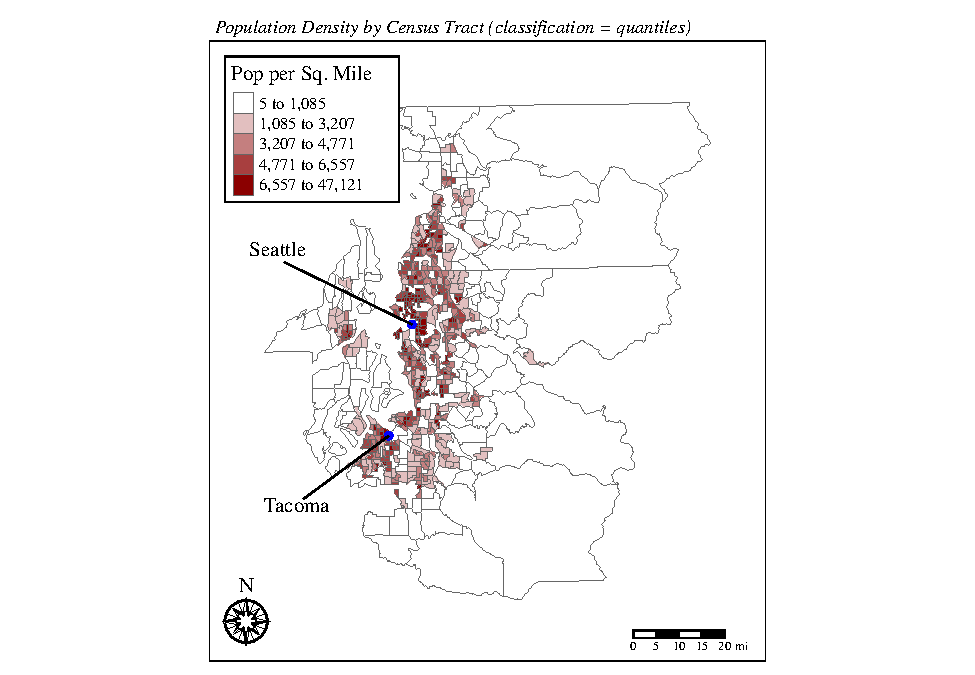
\includegraphics{transit-hotspots-PSRC_files/figure-latex/unnamed-chunk-5-1.pdf}
\caption{Sources: US Census ACS 2022 5-year estimates, Puget Sound
Regional Countil, Cities and Towns of the US 2014, via Stanford
University; Classification = jenks}
\end{figure}

As expected, population density is much higher in tracts close to the
two cities (and throughout the generally-urban corridor between them).
Again, visually comparing this pattern to the one seen for mass transit
percentage, a lot matches up. This is not a perfect correspondence, of
course.

\newpage

\begin{figure}
\centering
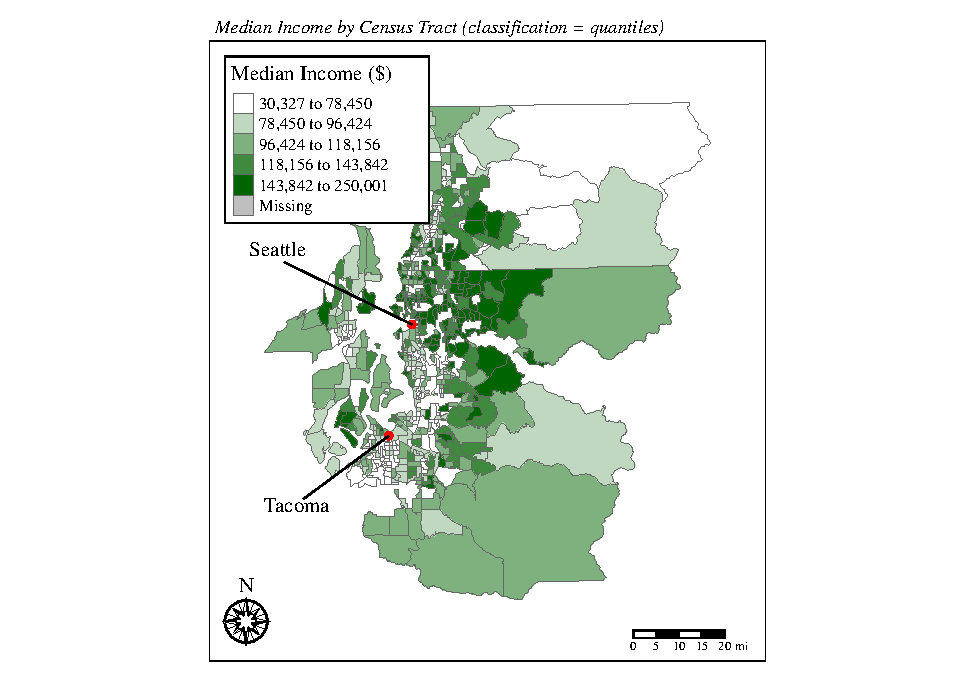
\includegraphics{transit-hotspots-PSRC_files/figure-latex/unnamed-chunk-6-1.pdf}
\caption{Sources: US Census ACS 2022 5-year estimates, Puget Sound
Regional Countil, Cities and Towns of the US 2014, via Stanford
University; Classification = jenks}
\end{figure}

I find this map to be particularly interesting. Although it is not
incredibly easy to compare this spatial pattern to the mass transit
percentage one, I will direct your attention to the high-income area
just East of Seattle. Comparing to the transit map, we can see a pretty
obvious negative association between income and transit percentage. This
provides an initial piece of evidence in favor of the hypothesis that
higher income tracts are likely to have lower transit usage. In the same
vein, a visual inspection of the tracts directly to the south of the
Seattle marker shows an area of comparatively low median income. Again,
cross-referencing this with the transit map, we can see this is an area
of relatively high transit usage.

\begin{figure}
\centering
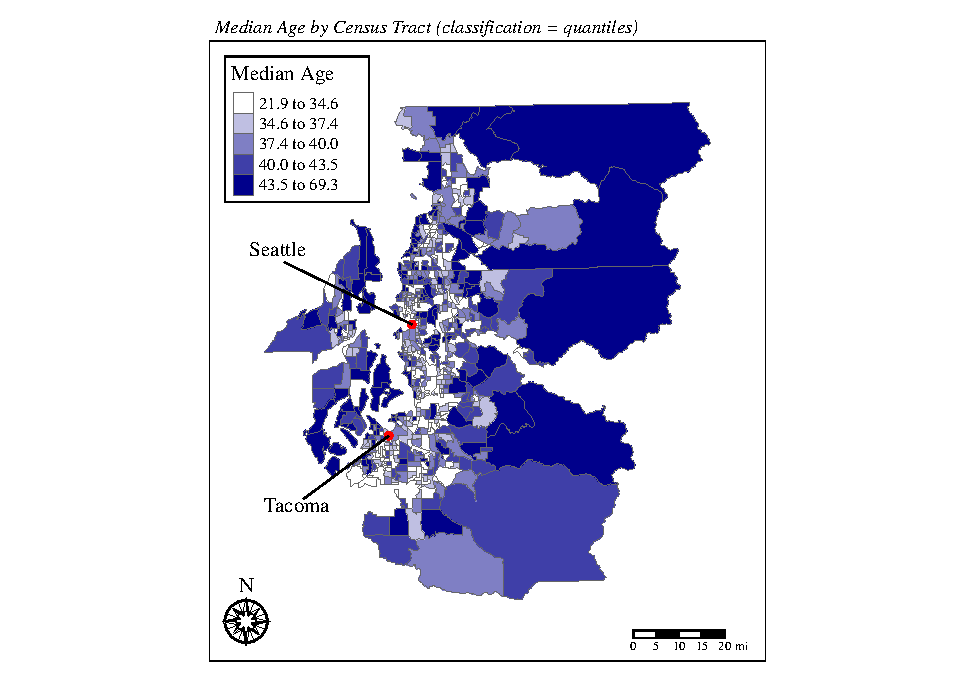
\includegraphics{transit-hotspots-PSRC_files/figure-latex/unnamed-chunk-7-1.pdf}
\caption{Sources: US Census ACS 2022 5-year estimates, Puget Sound
Regional Countil, Cities and Towns of the US 2014, via Stanford
University; Classification = jenks}
\end{figure}

\textbf{INSERT SOURCES}

\end{document}
